\subsection{Analysis of Distance Estimates}

\subsubsection{Model / Manual Distance Comparison}\label{subsubsec:distance_comparison}

In this section, the precision and accuracy of the distance estimates generated using the
four configurations of the distance estimation pipeline (outlined in
Section~\ref{subsubsec:configuratons}) are evaluated.
In order to for these data to be analysed, the estimates are benchmarked against their
corresponding manual distance estimates (supplied with the dataset), thus these estimates
use detection frames originating from the manual sample (Section~\ref{subsubsec:sampling}).

Ideally, each and every manual distance should be joined to its corresponding modelled
distance estimate; however, due to the absence of any frame-position data associated
with the manual annotations, automating this using traditional algorithms is impossible
in circumstances where multiple chimps are captured in a single frame.
This is because when multiple individuals are detected, there is ambiguity in regard to
which distance a given modelled distance should be joined to.
Moreover, approaching this task manually is extremely labour-intensive and was therefore
outside the scope of this project.
As a result, this analysis focuses on distance comparisons associated with frames capturing
only a single individual.

\begin{figure}[htbp]
    \centering
    \vspace{1cm}
    \includegraphics[width=1.01\textwidth]{body/analysis/assets/distance_graphs/averages3}
    \caption{Distance Comparison}
    \label{fig:distance_comparison}
\end{figure}

\clearpage

\begin{figure}[htbp]
    \centering
    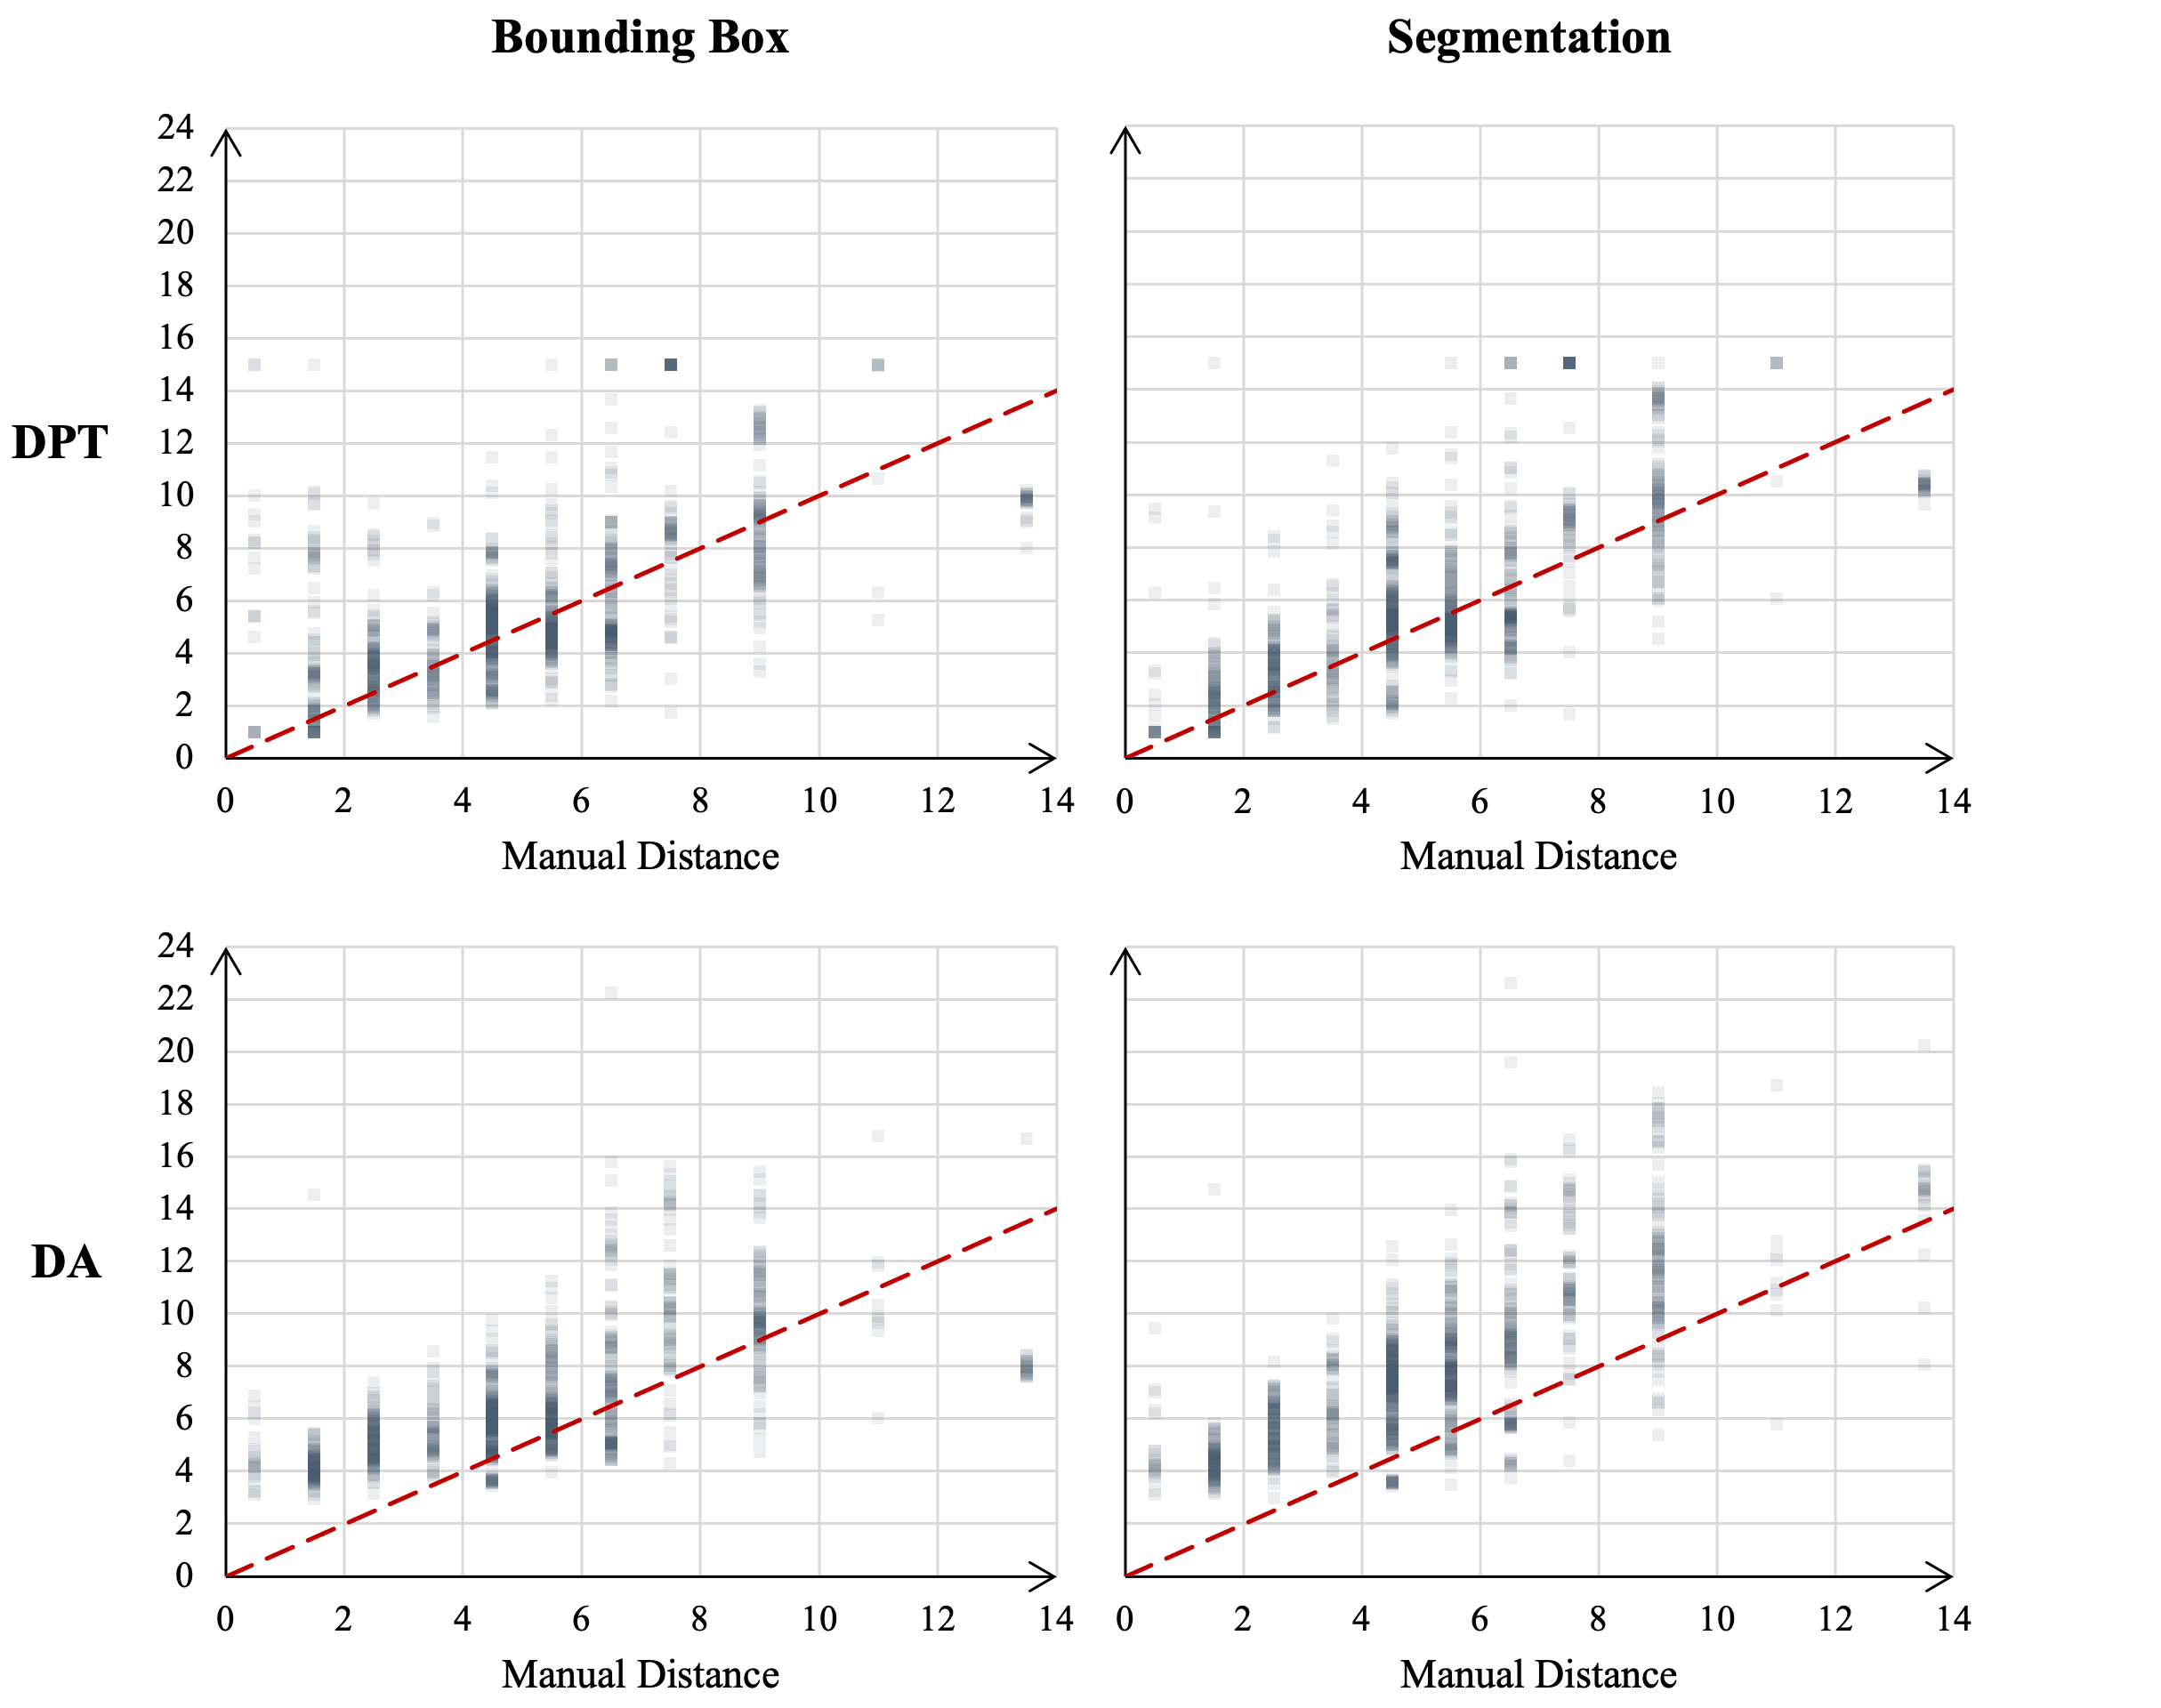
\includegraphics[width=1.01\textwidth]{body/analysis/assets/distance_graphs/spread}
    \caption{Spread Comparison}
    \label{fig:spread_comparison}
\end{figure}

How does parameterisation affect the estimates

\clearpage

\subsubsection{Error Analysis}

\begin{table}[htbp]
    \centering
    \caption{Errors}
    \label{tab:distances}
    \begin{tabular}{ccccc}
        \textbf{Method} & \textbf{$\Delta_{average}$ / m} & \textbf{MAE / m} & \textbf{RMSE / m}
        & \textbf{Statistical Difference} \\
        \midrule
        DPT, BBOX & 0.586 & 1.81 & 2.66 & YES \\
        DPT, SEG  & 0.836 & 1.70 & 2.45 & YES \\
        DA, BBOX  & 1.49  & 2.03 & 2.62 & YES \\
        DA, SEG   & 2.80  & 3.00 & 3.52 & YES \\
    \end{tabular}
\end{table}

\clearpage

\begin{figure}[H]
    \centering
    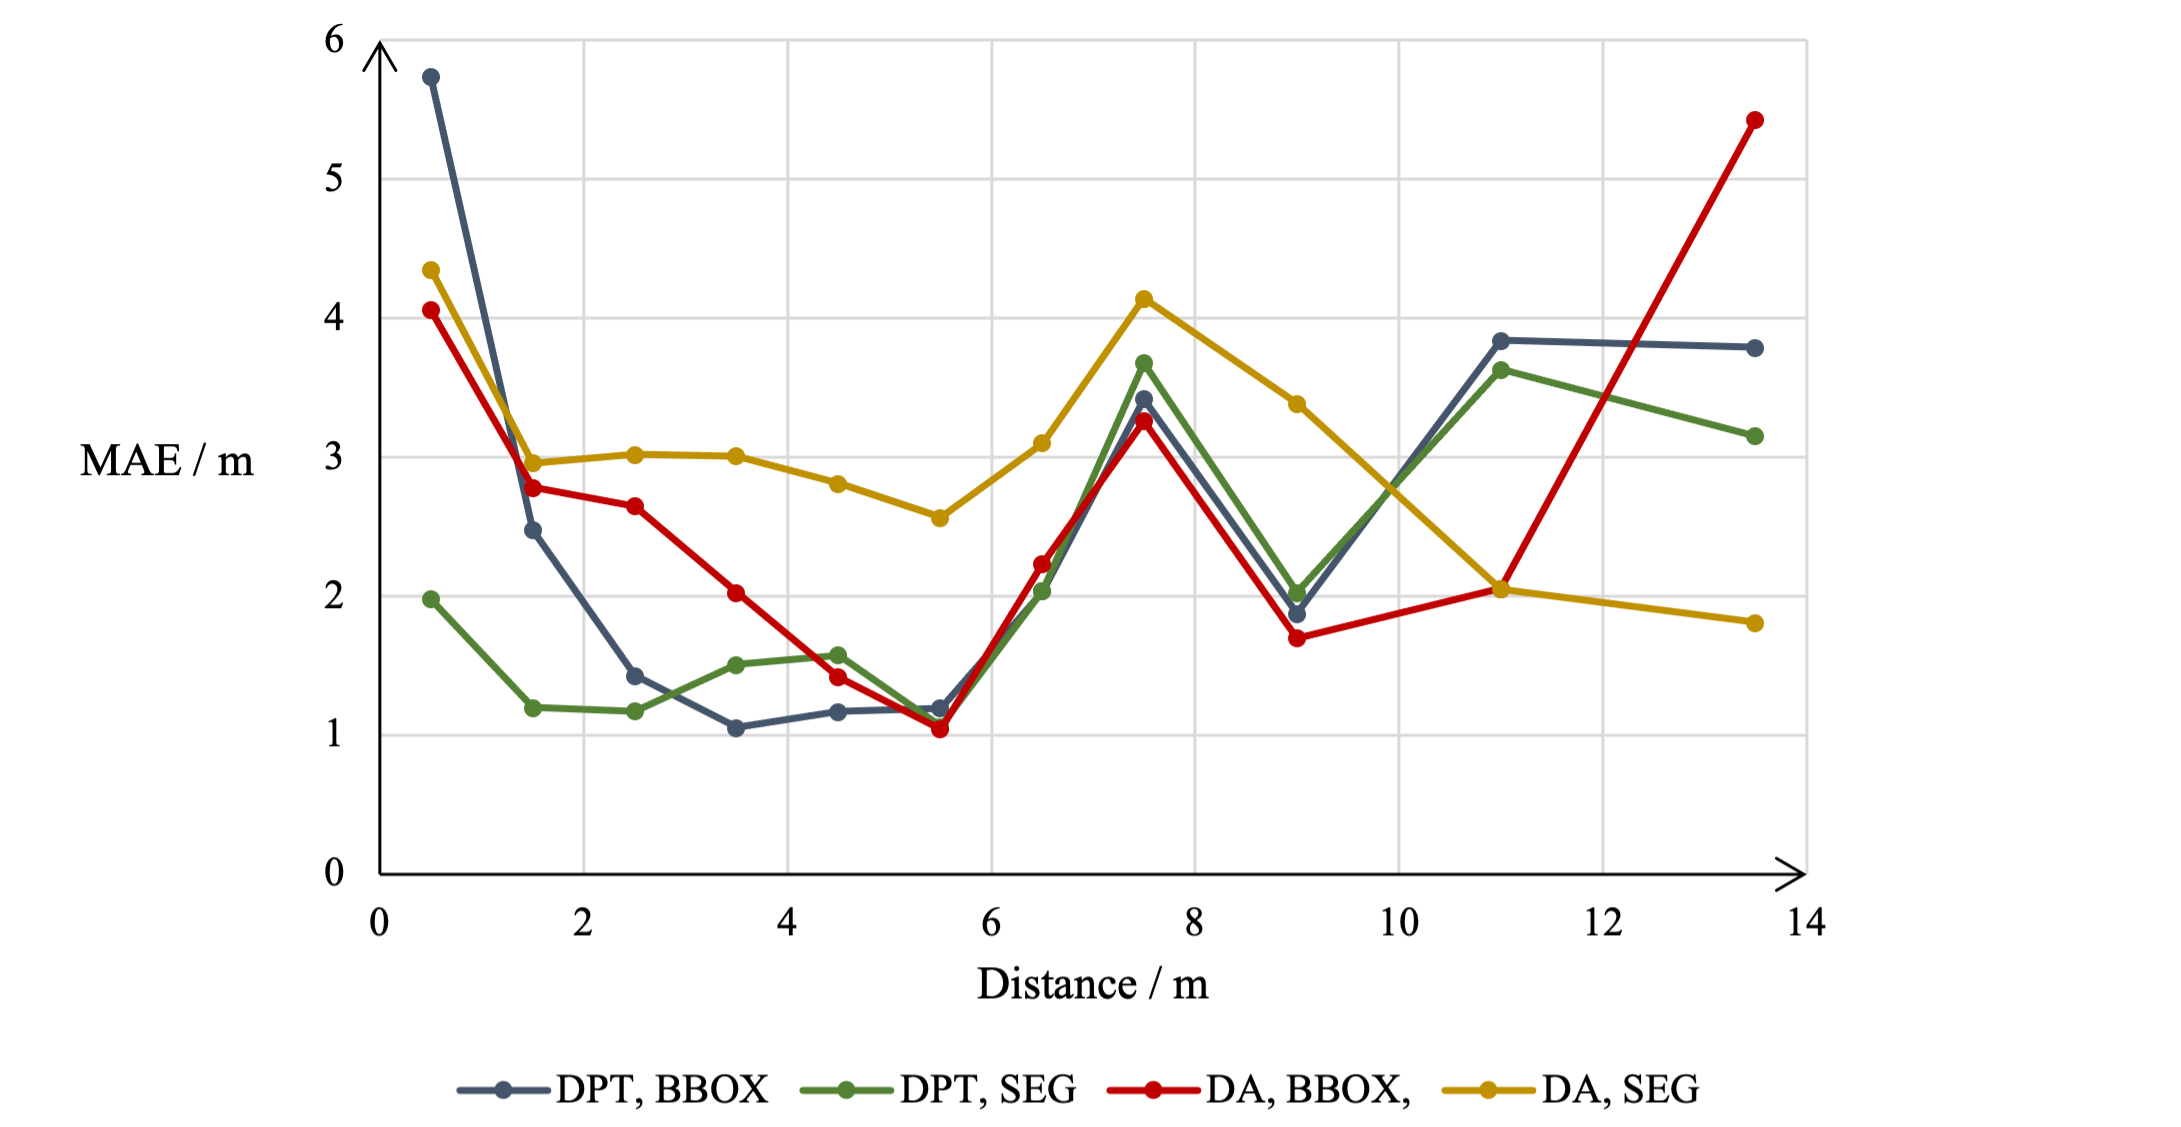
\includegraphics[width=1.01\textwidth]{body/analysis/assets/errors/MAE}
    \caption{Mean Average Error}
    \label{fig:mae}
\end{figure}

\begin{figure}[H]
    \centering
    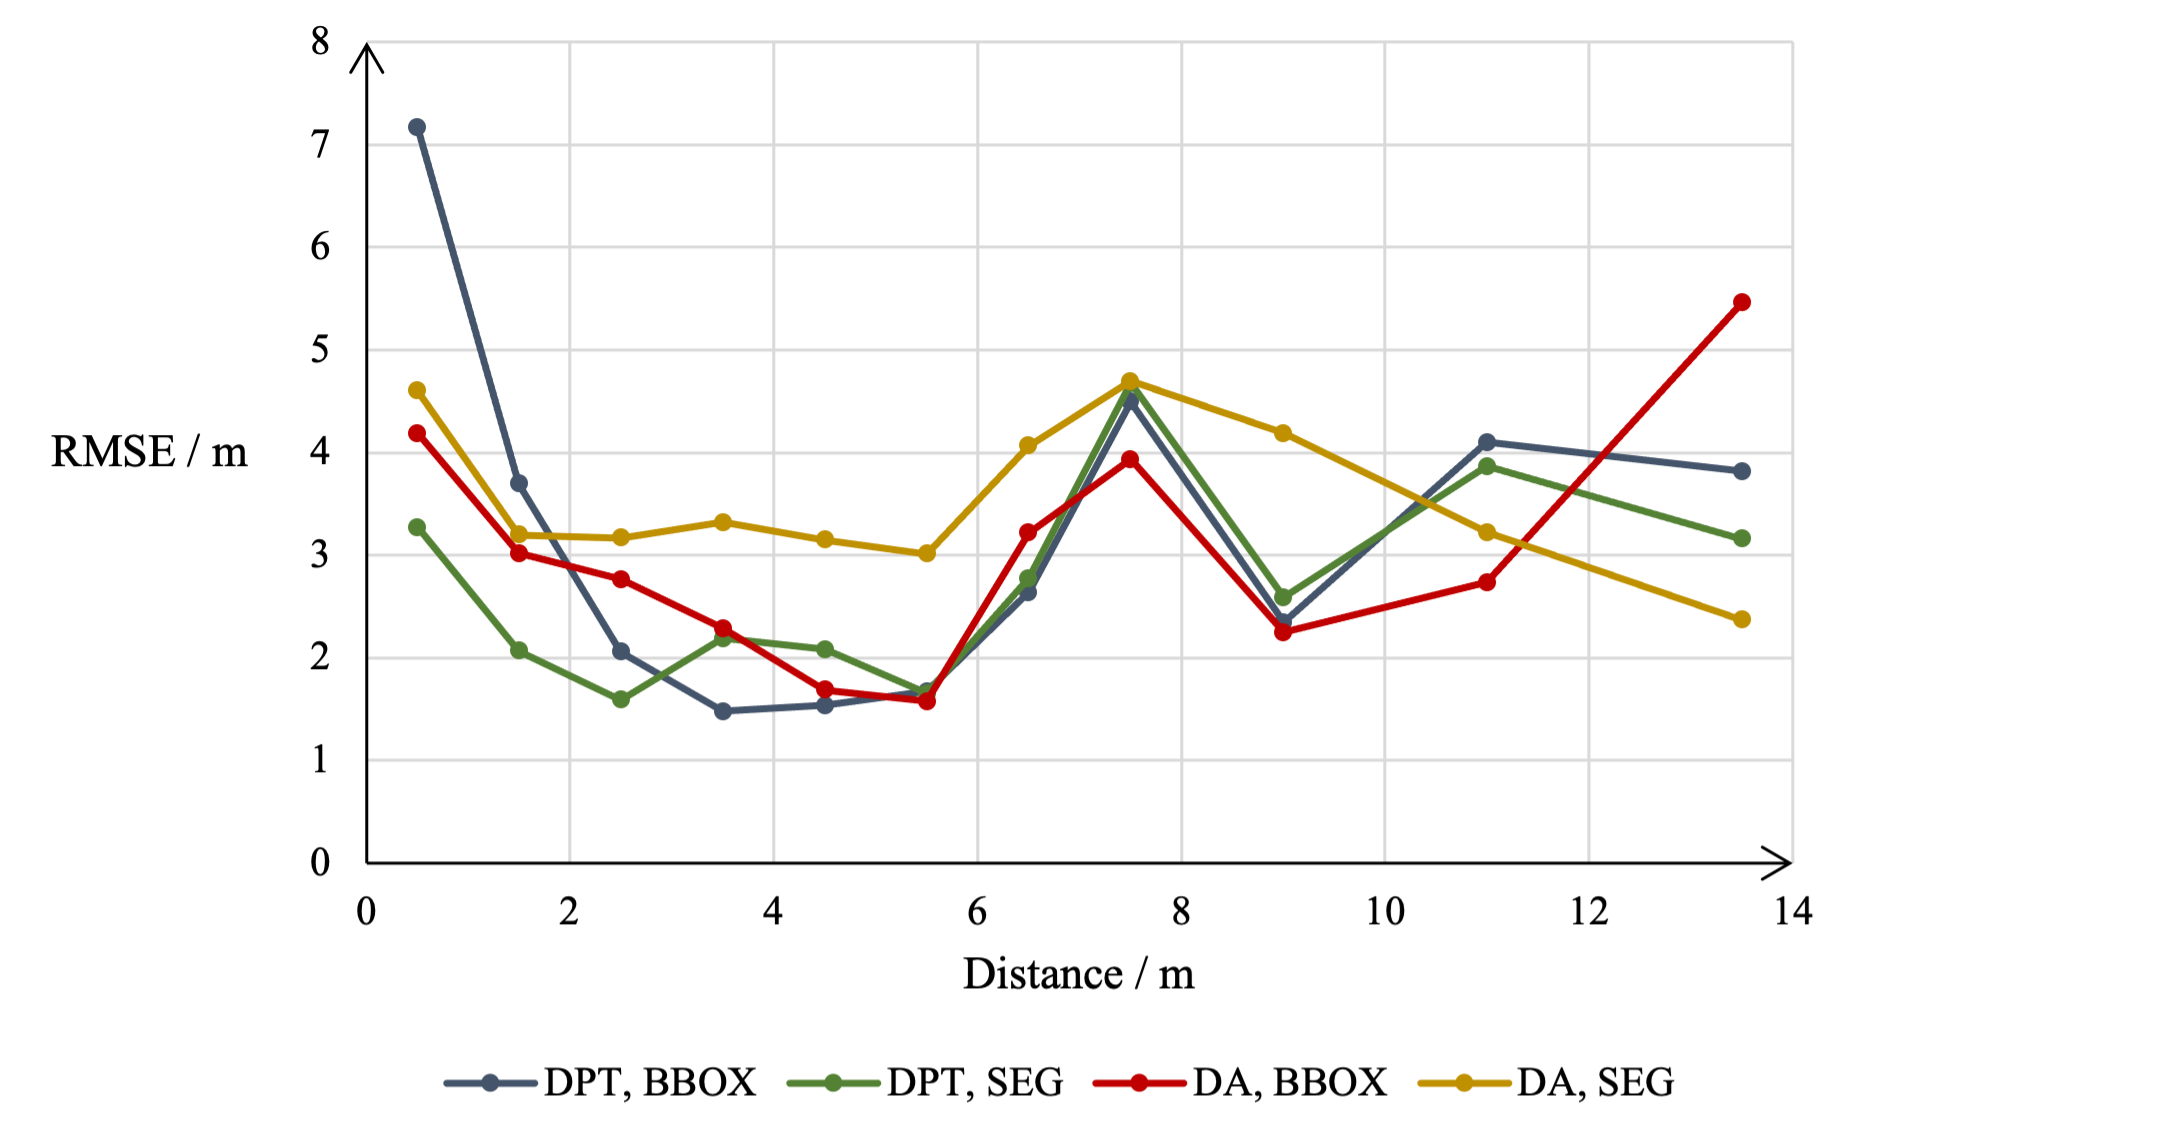
\includegraphics[width=1.01\textwidth]{body/analysis/assets/errors/RMSE}
    \caption{Root Mean Squared Error}
    \label{fig:rmse}
\end{figure}

\clearpage


\subsubsection{Qualitative Analysis}
depth map diagrams
close/far failure cases, sweet spot

\subsubsection{Effects of Varying Calibration}